\section{Considerations}

Design of the metrics unit can be split into two components: the design of the
standalone metrics data and computation component, and integration of the data
and computation component into the object of importance: the \gls{real-time}
\gls{pipeline}.

\subsection{Data and Computation Component}

Design of the data collection and metric computation unit required consideration
of multiple criteria including: the data structure to be used to contain
samples, the structure of the samples, thread safety, and preventing
side-effects.

\subsubsection{Component Design}

The standalone metrics component was required to satisfy multiple criteria. The
component needed to be minimally invasive, when pushing data to the component
from the pipeline there should be minimal slowdown. The component needed to be
thread-safe as multiple pipelines exist and interact with the metrics component
at the same time, in addition to the command-line interface retrieving the metrics
data. There was also the necessity of consistency in the data returned, as
the metrics component returns multiple independent metrics when the metrics are
requested. Additionally, the component must exemplify the object-oriented
programming best-practice of encapsulation, providing as little information
about it's inner workings as necessary. The first iteration of the metrics
framework proved the general idea was possible and meaningful results were
returned. A second iteration was produced to better meet the goals outlined
above. This second iteration was designed to provide improved reliability by
detecting faults, such as divide-by-zero calculations, before they occurred, and
readability of the source code such that the software could be more easily
maintained. The general design of the framework is a metrics object owned by
each \gls{pipeline}, which handles storing, and computing of the metrics, and
printing of the metrics snapshot. Interaction with these metrics objects occurs
through callbacks already present in the \glspl{work-unit} passing through the
processing \gls{pipeline} in addition to other related components of the
pipeline.

\subsubsection{Storing Samples}

The data structure to be used was an important consideration as it would act as
the backbone of the metrics component, storing samples that get pushed to the
object and later retrieval of those samples for processing. The structure
required must be efficient in both submission and retrieval of samples. The
\gls{rolling} nature of the metrics component allowed the data structure to be very
limited in space, as new samples could overwrite old samples when the size of
the \gls{rolling} window was reached. Structures considered would all be
implemented in the C++ language the existing code-base was primarily
comprised of. Structures considered were C++ vectors, C++ lists, and circular
buffers from the Boost \gls{library} \cite{boost:circularbuffer}.  Vectors
support fast retrieval in constant time (\textit{i.e.}, $O(1)$: the times stated
are all \gls{bigo} times) and insertion and removal of elements at the end of
the structure in amortized constant time (constant time over a large sample,
only deviating from constant time in the infrequent event more memory must be
allocated). C++ lists also support fast linear traversal -- which is how the
metrics data is processed -- in constant time, and insertion in constant time.
Illustrated in Fig.~\ref{fig:ring_buffer}, Boost's circular buffer also supports
constant time access, and amortized constant time insertion; however, has a
greater ease of use than vectors or linked lists. Using a vector or linked list,
implementing the \gls{rolling} statistics window would require the programmer to
manage the window whether that's only looking at specific elements of the data
structure or managing the overwriting of elements. The Boost \gls{library}'s
circular buffer will create a buffer of set size and overwrite old elements to
insert new elements when that size is reached. As such Boost's circular buffer
(\lstinline|boost::circular_buffer|) was found to be the most fitting data
structure to store the samples in.

\begin{figure}
	\centering
	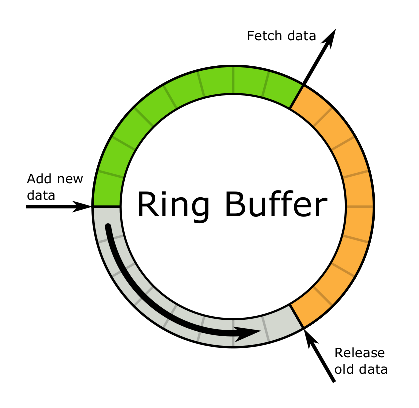
\includegraphics[width=0.5\columnwidth]{ring_buffer}
	\caption{Circular (ring) buffer}
	\label{fig:ring_buffer}
\end{figure}

\subsubsection{Sample Structure}

When storing samples, they had to be in a format that made computation of
relevant metrics easy and fast. An in-house library providing many basic
functionality including time values was initially used to implement the \gls{pipeline}
metrics. The initial successful iteration of the metrics component was on a
Linux platform using \gls{gcc} however when attempting to compile with
\gls{msvc} errors were encountered relating to the usage of the time values from
the general library.  As cross-platform compatibility was the ultimate aim of
this project it was then decided to implement the samples using Boost's Posix
Time library (\lstinline|boost::posix_time| and
\lstinline|boost::posix_time::time_duration|) \cite{boost:posixtime}. The use of
a specialized time object allowed easily storing event times and computing the
difference between stored times, both
important in calculating metrics such as the continuously computed rolling rate
of an event and discretely computed rates of events. When computing the
continuous metrics, every time a snapshot is generated the
\lstinline|boost::posix_time| samples of event occurrence times are
compared against the current time whereas in computation of the discrete metrics
only the time difference between event occurrences is known, updating only when
a new event occurs. The largest example of this distinction is the overflow rate
metric, which is continuously computed as overflows happen so rarely the metric
is more useful updating continuously; other metrics describe events that occur
more consistently and therefore are more informative when calculated discretely.

\subsubsection{Impact on Processing}

The impact of the metrics component on processing had to be minimized. Ensuring
unreasonable delays were not incurred by utilizing the metrics component had
large a part in shaping the design of the component. Since adding samples
happens in the callback of \glspl{work-unit}, running on the same thread as
processing, minimal delay was necessary. The result of this requirement was new
samples being added to the circular buffer and only when a metrics report is
requested are metrics calculated. This metrics request can occur in a
\gls{thread} other than a processing thread preventing the incurrence of
unnecessary slowdowns in processing.

\subsubsection{Thread Safety}
Since multiple processing \gls{pipeline}s will interact with the metrics object at a
time, it must be made thread safe. Additionally, when retrieving the current
value of the metrics updates must not be made to the values while calculations
are being executed. To solve these issues, a \gls{mutex} is used to serialize
access between threads. When retrieving current values, a snapshot of the
metrics is generated then returned to ensure consistency between when the values
are requested and when they are displayed. The use of a snapshot ensures the
values are constant between when they are requested and when they are printed.
Ensuring consistency between metrics (such as when computing mean and max from
the same samples) was achieved by acquiring a lock on the metric object's mutex,
ensuring no updates can be made until the \gls{mutex} is unlocked when
computation of all the current values is complete. When an update is being made,
the mutex is also locked and the current values can only be computed after the
lock is released.

\subsection{Pipeline Integration}

A challenge encountered integrating the new metrics component was ensuring
minimal changes were made to the processing \gls{pipeline}, and any changes made
to integrate the metrics component with the \gls{pipeline} did not break current
functionality of the \gls{pipeline}. Integrating the metrics component into the
\gls{pipeline} required utilizing existing callbacks in the \gls{pipeline} and
adapting \glspl{work-unit} to provide the necessary callbacks to the metrics
component. A \gls{work-unit} provides a callback function after it has finished
execution. The metrics framework utilizes this callback to signal the duration
of queuing and execution. Additional hooks were necessary to signal queue
overflow and submission instances which are used respectively for both overflow
rate and count, and submission rate.  The metrics component receives
\lstinline|boost::posix_time| \glspl{instance} when the time an event occurred
is needed such as for queue overflow and submission time, and
\lstinline|boost::posix_time::time_duration| \glspl{instance} when only the time
difference between events is required. The decision to use either depends on
whether the metric is continuously or discretely updated. By utilizing existing
callback functionality minimal changes were made to any \gls{pipeline}
components when integrating the metrics component.
